\section*{\revise{Supplementary Material}}
\label{sec:SupplementaryMaterial}

\subsection*{\revise{Details of \ac{STDPH} and \ac{NMF} experiments on retrosplenial cortex}}

\revise{Alexander and Nitz \cite{AlexanderNitz2015} investigated the spatial reference frame(s) to which retrosplenial cortical activity is anchored. In their experiments, six Long-Evans rats traversed a W-shaped track that occupied two distinct positions in the recording room, referred to as track positions $\alpha$ and $\beta$, which varied by recording session. The track was composed of two sets of action sequences depending on the direction of traversal (outbound or inbound trials). Outbound and inbound runs were made up of opposite turn sequences (left-right-left (LRL) and right-left-right (RLR), respectively. The manipulation of turn sequence, route, and track position allowed the assessment of neural sensitivity to the \textit{allocentric}, \textit{egocentric} and \textit{route-based} reference frames by comparing the observed firing patterns of electrophysiologically recorded neurons by the rat's position with respect to the route, the room, and the action being performed. In total, 243 neurons were recorded over 71 recording sessions, with measures taken to ensure maximum independence between the neurons that were recorded in each session. Each session had approximately 20 trials per condition (track position by direction of traversal). Additionally, Alexander and Nitz \cite{AlexanderNitz2015} recorded relevant behavioral data concurrently with neuronal firing patterns for each trial, including head direction (HD), position in X-Y coordinates (Pos), linear velocity (LV), and angular velocity (AV).}

\begin{figure}[!h]
	\centering
	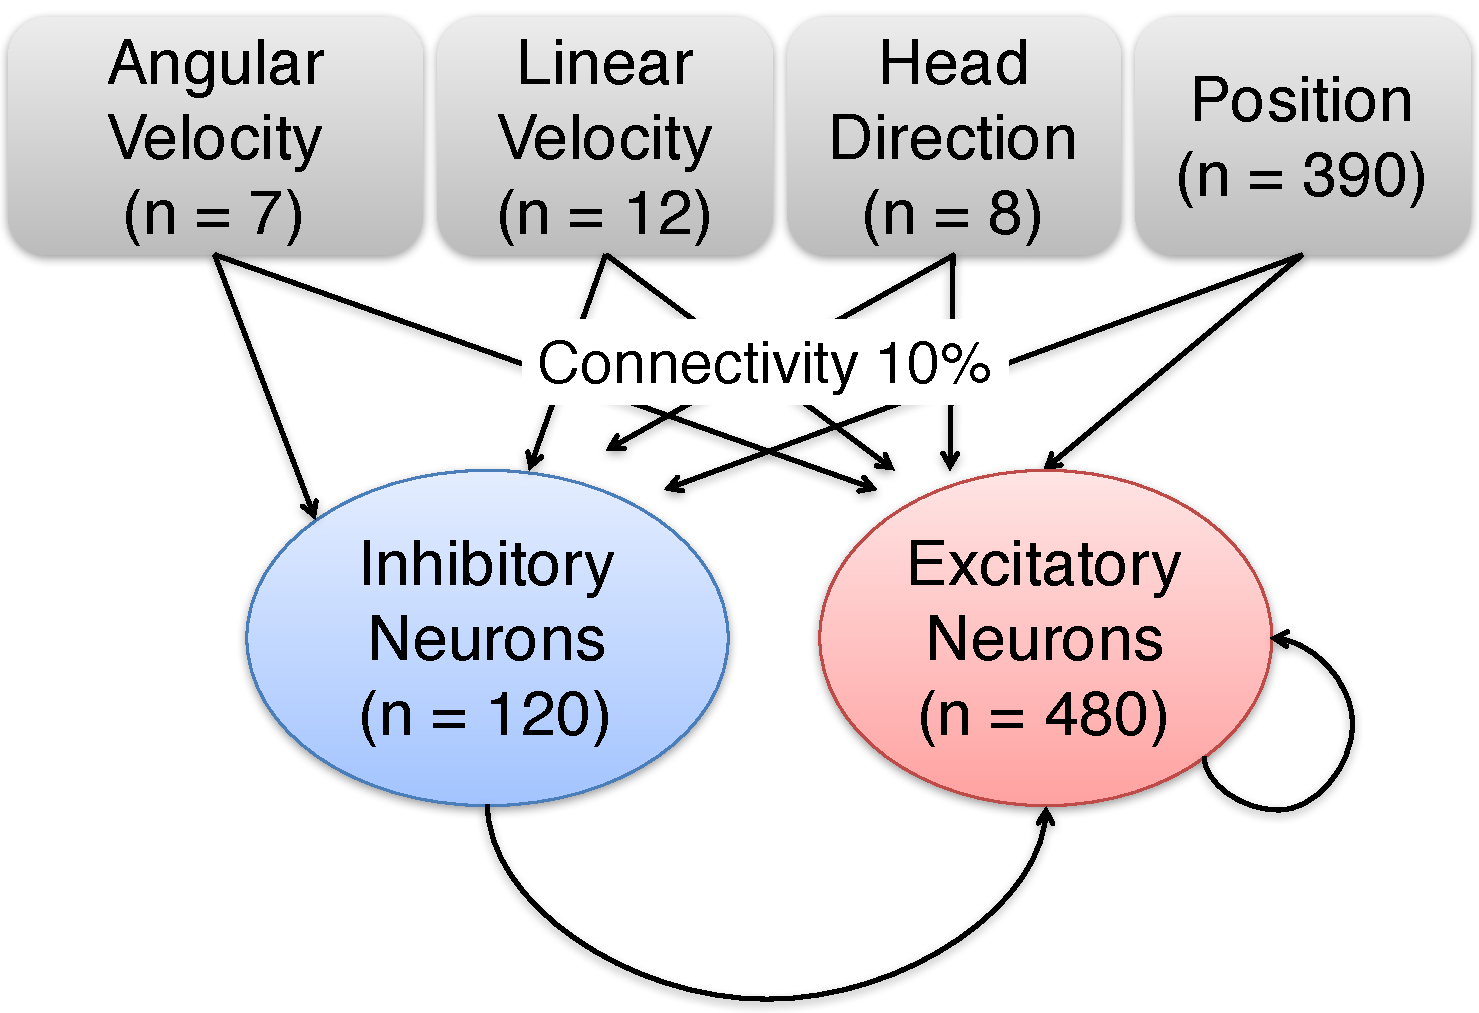
\includegraphics[width=\textwidth]{RSC_NetArch}
    \caption{\revise{The spiking neural network had four input groups and a total of 417 excitatory input neurons (390 neurons for position, 8 for head direction, 12 for linear velocity, and 7 for angular velocity). There were a total of 600 output Izhikevich neurons, 80\% excitatory (480 neurons) and 20\% inhibitory (120 neurons). Network connectivity was set at 10\% probability across all connections (inp->inh, inp->exc, inh->exc, and exc<->exc), and each connection type was governed by its own STDPH curve (excitatory STDP on the inp->exc, inh->exc, and exc<->exc connections, and inhibitory STDP on the inp->inh connections). The total size of the network was 1,017 neurons.}}
	\label{fig:RSC|spikingarch}
\end{figure}

\revise{Using the experimental data collected in these experiments, our group used an evolutionary strategy to evolve \revise{paramenters corresponding to STDPH and homeostasis in a population of} spiking neural networks (SNNs) that could replicate the functional, behavioral, and population responses observed in the electrophysiologically recorded data in response to the recorded behavioral metrics HD, Pos, LV, and AV  \cite{Rounds2016,Rounds2018}. 
Each network contained 600 neurons (480 excitatory and 120 inhibitory Izhikevich neurons \cite{izhikevich2003simple}). Each trial consisted of 200 bins, each associated with a specific combination of these four inputs. The recorded values were encoded using cosine and Gaussian tuning curves that were subjected to a Poisson process to produce spiking inputs. The population was allowed to evolve over 50 generations, with convergence occurring by approximately the 20th generation. Synthetic neural activity was averaged across trials for each track position/traversal combination and then correlated with the 243 electrophysiologically recorded neuronal firing patterns. For each of the electrophysiologically recorded neurons, the synthetic neuron with the highest-correlated firing pattern was assigned as a match for that neuron. No duplicate matches were allowed - a neuron could be matched only once. Each SNN in the population was evaluated according to a fitness function that measured the sum of the highest correlations between neurons, with a penalty for overly high average maximum firing rates for the synthetic neurons to ensure a stable firing regime. The networks consistently converged to a fitness value of 105.93 $\pm$ 0.91 (arbitrary units), or an average correlation of Pearson's \textit{R} = 0.43 per neuron (high correlations by experimental standards). For further details on experimental methods, see \cite{AlexanderNitz2015,Rounds2016,Rounds2018}.}

\revise{In the \ac{NSC} experiment, the idealized \revise{neural activity}
was used to construct a matrix of training data associated with each of the four recorded `features' (i.e., linear velocity, angular velocity, head direction, and position), to which \ac{NMF} was applied. We tested a range of parameters for the number of basis vectors to which the input matrix would be reduced; ultimately, 30 basis vectors best captured the results of the experimental data.}

\revise{We found that the activity patterns of both \ac{NSC} and \ac{STDPH} model neurons could replicate the neuronal response properties and population activity seen in the electrophysiologically recorded neurons in the dataset (Fig.~\ref{fig:NMF|RSC}A, B, C, left); that is, the model neuron activity could be classified into three broad categories,
with remarkably similar population statistics to rat \ac{RSC} 
\cite{AlexanderNitz2015} \emilyNote{may or may not want to keep this note explaining functional type distribution differences}
(note: while STDPH functional neuron type distributions differ from those observed in the experimental data and the \ac{NMF} model, we believe this is not a concern due to the high rate of functional remapping observed in the evolved SNNs \cite{Rounds2018}):
1) Turn-sensitive, no modulation neurons responded whenever the animal made a left or right turn
   on the track (light gray);
2) Turn-sensitive, route modulation neurons responded whenever the animal made a turn on a specific position along
   the route, independent of allocentric location (dark gray); and
3) Turn-insensitive neurons that did not reflect turning behaviors or actions performed by the rats,
   but nonetheless exhibited complex and robust firing patterns (white). This set of neurons appear to encode information related to position in allocentric space with modulation by other variables. In addition, both \ac{NSC} and \ac{STDPH} model \ac{RSC} produced simulated neurons whose combined population activity could be used to predict the agent's location on a route with respect to the allocentric frame of reference. Population activity patterns could also disambiguate the agent's location within routes that occupied different locations in the room, consistent with findings of population behavior in the biological RSC \cite{AlexanderNitz2015}.}
  
